% !Mode:: "TeX:UTF-8"

\BiChapter{基于词典或知识库的方法与集成学习方法}{}
\label{c:ensemble}
词典或知识库是一种描述词语语义的语言学资料。这里的词典并不像我们常用的词典那样使用自然语言解释词语,它会将词语组织成一定的结构,并且使用形式化的方式进行描述。这就为词语的语义提供了一种计算机容易理解的表示形式。

在英文方面,最著名的词典或知识库是普林斯顿大学开发的 WordNet\citeup{Miller1995}。而在中文方面,则有董振东教授开发的知网(HowNet)与梅家驹等人开发的同义词词林。后者经过了哈尔滨工业大学信息检索实验室的改进,形成了同义词词林扩展版。

集成学习是一种将多个个体学习器进行组合,而获得更高性能的学习器的机器学习方法。这种方法通常可以得到好于任何一个个体学习器的性能。

主流的集成学习方法分为三种,分别被称为 boosting、bagging 和 stacking。其中,boosting 使用迭代方法训练一系列学习器,每次迭代都根据上一个学习器的输出改变样本的权重,使得上一个学习器分类错误的样本获得更高权重;Bagging 使用一种有放回的“自助采样”方法生成多个样本集,用每个样本集训练一个基学习器,并使用投票方式将这些学习器的输出进行组合;Stacking 则使用一个额外的学习器来组合基学习器的输出。本课题中使用 stacking 方法进行集成学习。

本章将会给出一种基于同义词词林扩展版的词语相似度计算方法,并使用集成学习的方法来结合本文中先前介绍过的各种方法。由于二者结合非常紧密,故合并在一章内介绍。

\BiSection{原理介绍}{}
\BiSubsection{同义词词林扩展版}{}
最初版本的同义词词林包含 53859 个词条,随着大家对中文使用习惯的变化,有 14706 个词条的使用频率降低,成为了罕用词与非常用词。同义词词林扩展版删除了这些词语,并且增补完善了一定数量的词语,使得最终的词条数量达到了 77343 条。

在结构上,同义词词林扩展版将词条分类组织为一个树状结构,如图 \ref{f:cilin layers} 所示。分类的层次共有 5 层,随着层次的增加,词语语义的划分越来越细。第五层的词类称为原子词群。一个原子词群中的词语可能是同义词,可能是互相相关的非同义词,也可能一个原子词群中仅有一个词语。同一个词语可能同时出现在多个不同的原子词群中。这意味着这个词语是一个多义词。原子词群的编码方式如图 \ref{f:cilin code} 所示,其中,“=”表示一个原子词群是同义词,而“\#”表示一个原子词群是同类词语,“@”表示原子词群内只有一个词语。

\begin{figure}[h]
	\centering
	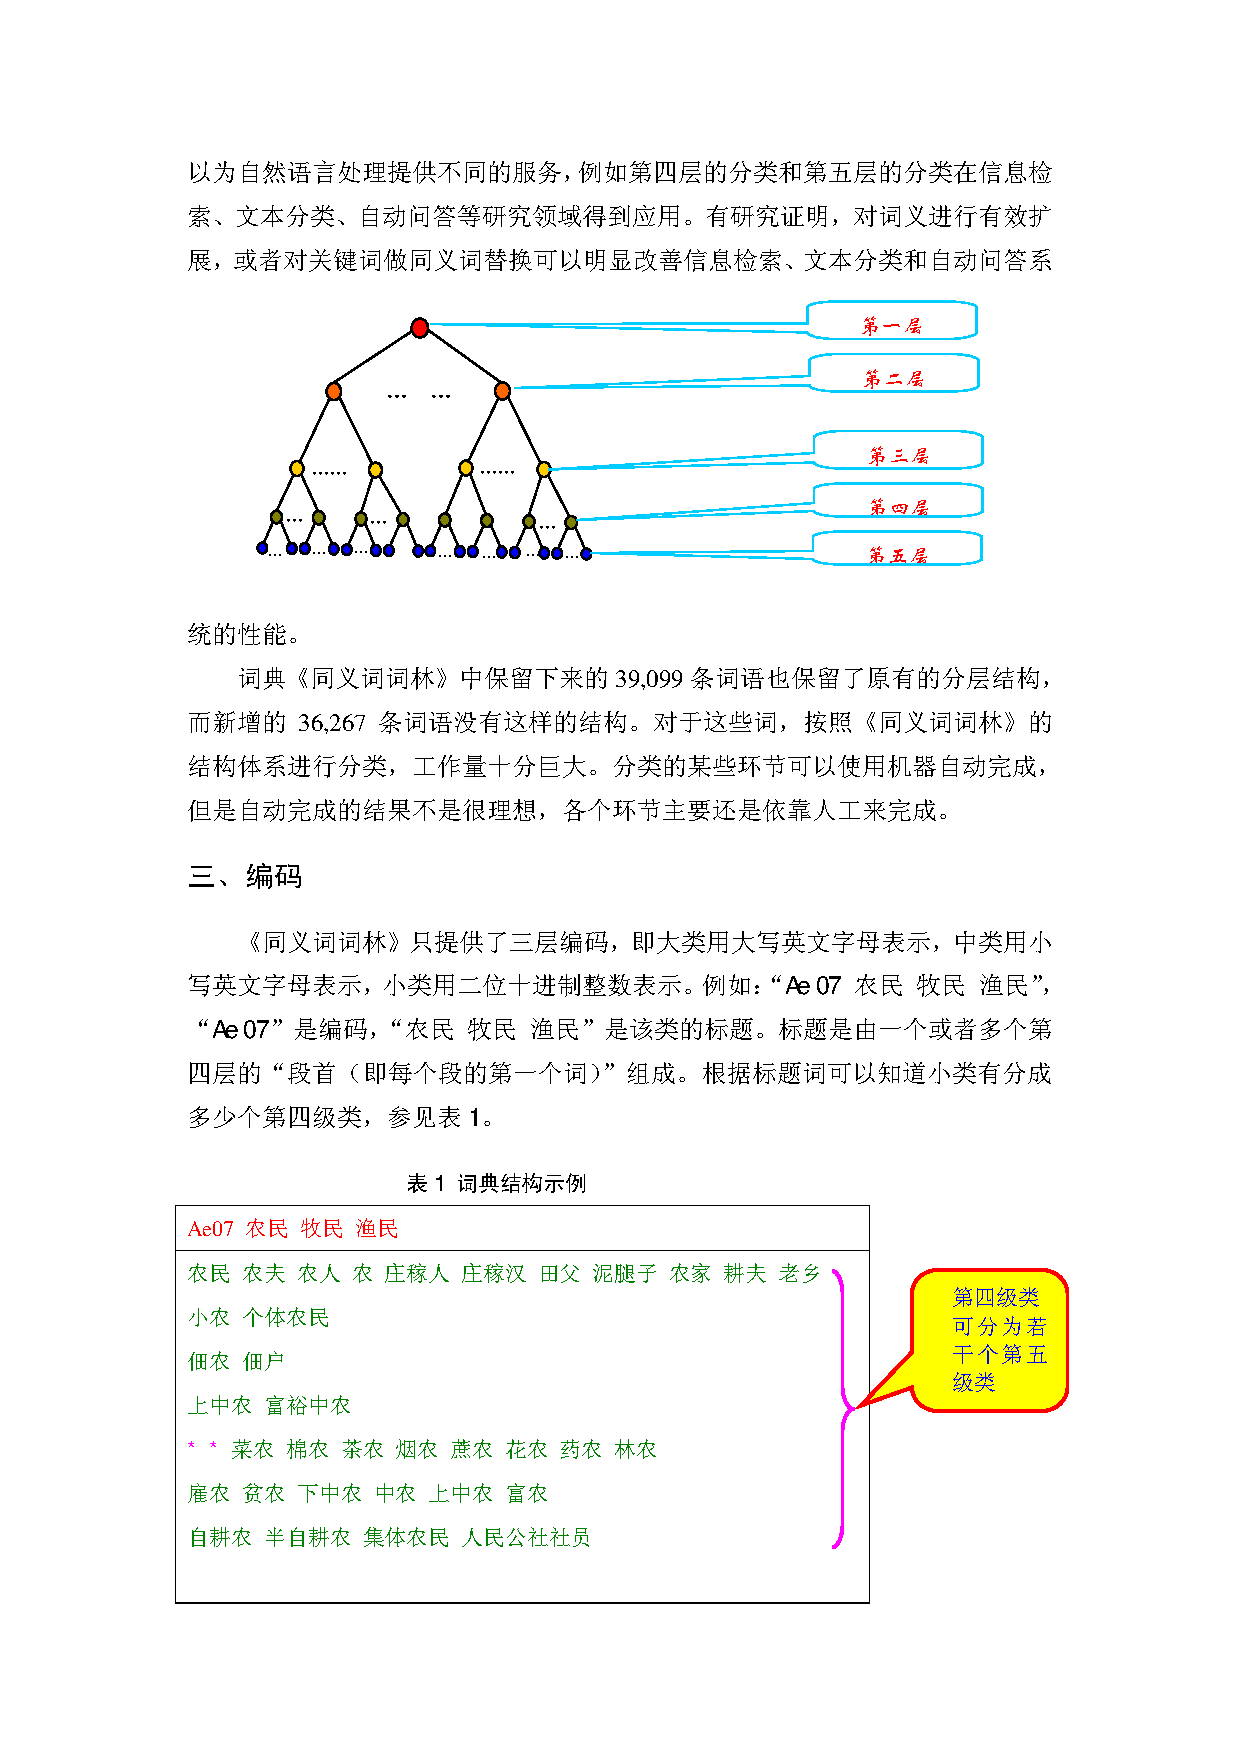
\includegraphics[trim={4.3cm 20.1cm 4.3cm 5.05cm},clip]{Cilin-layers}
	\caption{同义词词林扩展版的结构(来自同义词词林扩展版说明)}
	\label{f:cilin layers}
	\vspace{-1em}
\end{figure}

\begin{figure}[h]
	\centering
	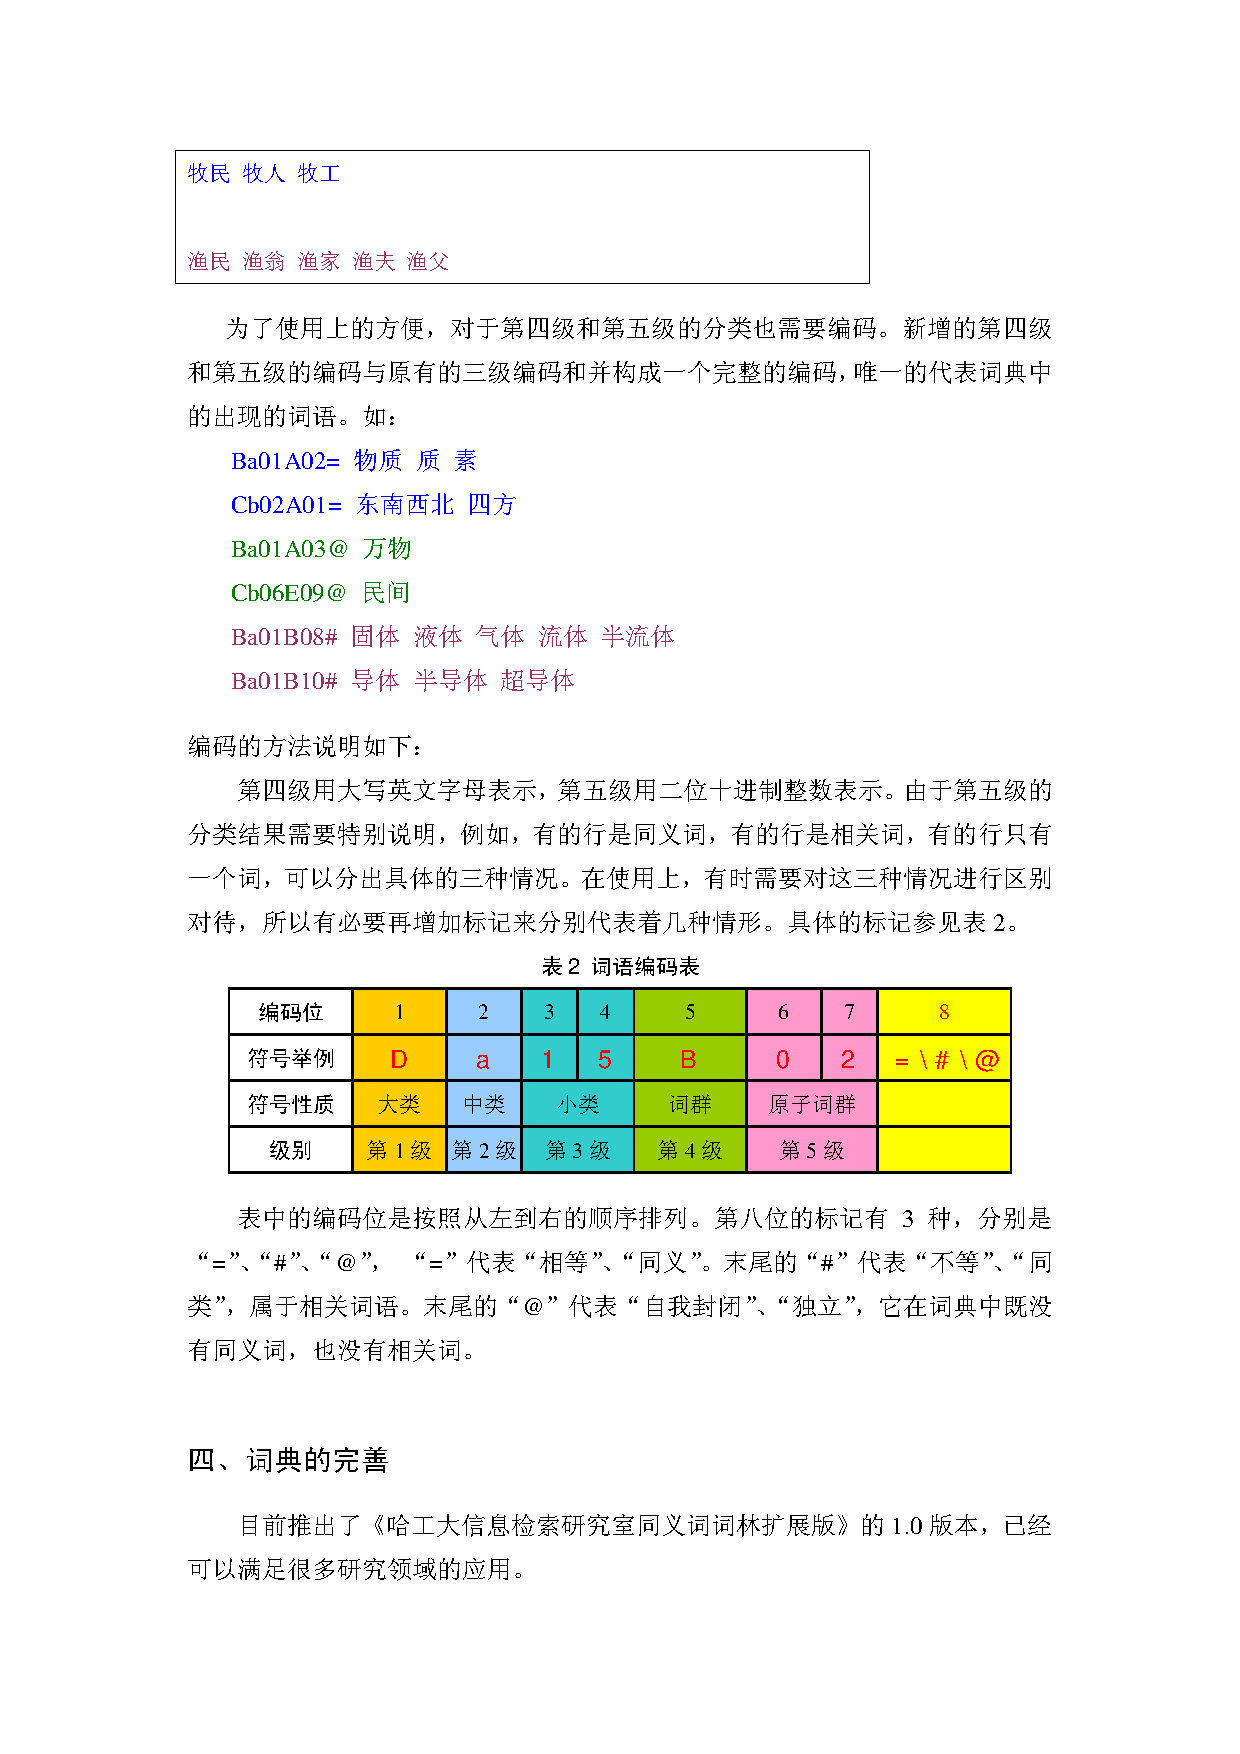
\includegraphics[trim={3.85cm 9.83cm 3.85cm 16.73cm},clip]{Cilin-code}
	\caption{原子词群的编码方式(来自同义词词林扩展版说明)}
	\label{f:cilin code}
	\vspace{-1em}
\end{figure}

\BiSubsection{Stacking 方法}{}
在上文中提到的三种集成学习方法中,stacking 方法是唯一一种具有集成异构的学习器的方法。由于本课题需要集成来自不同机器学习方法的结果,因此必须使用这种方法。Stacking 方法用一个学习器来组合其它学习器的输出。其中,被组合的学习器称为初级学习器 $M_i$,而用于组合的学习器称为次级学习器 $M_\text{e}$。

设集成学习系统的输入的特征为 $x$,而标注为 $y$,则每个初级学习器的训练过程与一般的机器学习过程相同。每一个初级学习器使用同样的特征与标注独立地进行训练,即训练目标为 $M_i(x) \rightarrow y$。训练完成后,每个初级学习器都会给出对标注的一个预测 $M_i(x) = y'_i$。

次级学习器 $M_\text{e}$ 则以初级学习器的输出 $y'_i$ 作为输入,其训练目标为 $M_\text{e}(y'_1, \dots, y'_n) \rightarrow y$。这样,次级学习器就起到了组合初级学习器的输出的作用。

在 stacking 方法中,每个初级学习器通常是用不同的方法构造出来的,这意味着初级学习器的数量不会很多(例如本课题中仅有三个,人工构建出大量的初级学习器的工作量是难以估量的)。于是,stacking 方法一般会使用相对较为简单的机器学习方法。本课题中分别尝试使用线性回归、岭回归与 LASSO 三种方法构造次级学习器。

\BiSubsection{线性回归}{}
线性回归是最为简单的回归方式之一,它使用一个线性函数产生对标注值的预测。假设我们有一个数据集 $\bigl\{(x_1, y_1), (x_2, y_2), \dots, (x_n, y_n)\bigr\}$,其中 $x_i \in \mathbb{R}^m, y_i \in \mathbb{R}$。线性回归具有如下的形式:
\begin{equation}
y'_i = \beta^\intercal x_i + b
\label{e:linear regression}
\end{equation}
其中,系数 $\beta$ 与置偏 $b$ 都是线性回归的系数。

线性回归的最优解很容易通过最小二乘法得到。最小二乘法令预测值与实际值之差的平方和最小,即:
\begin{equation}
(\beta^*, b^*) = \argmin_{(\beta, b)} \sum_{i = 1}^{n} (y_i - y'_i)^2
\end{equation}

将公式 (\ref{e:linear regression}) 中的变量进行一些变形,设:
\begin{align}
	X &=
	\begin{pmatrix}
		x_1 & x_2 & \cdots & x_n \\
		1 & 1 & \cdots & 1
	\end{pmatrix}^\intercal \\
	Y &= (y_1, y_2, \dots, y_n)^\intercal\\
	\hat{\beta} &=
	\begin{pmatrix}
		\beta \\
		b
	\end{pmatrix}
\end{align}
则最小二乘法的目标变为:
\begin{equation}
\hat{\beta}^* = \argmin_{\hat{\beta}} (Y - X \hat{\beta})^\intercal (Y - X \hat{\beta})
\end{equation}

通过求导的方式,可以得到:
\begin{equation}
\hat{\beta}^* = (X^\intercal X)^{-1} X^\intercal Y
\end{equation}
即是线性回归的最优解。

\BiSubsection{岭回归与 LASSO}{}
在样本特征较多,而样本数量较少时,线性回归容易出现过拟合的问题。解决这个问题的方式是对模型参数添加规范化项。

如果规范化项为 L2 规范化,则称为岭回归:
\begin{equation}
\hat{\beta}^* = \argmin_{\hat{\beta}} \bigl((Y - X \hat{\beta})^\intercal (Y - X \hat{\beta}) + \lambda ||\hat{\beta}||^2_2\bigr)
\end{equation}

如果规范化项为 L1 规范化,则称为 LASSO :
\begin{equation}
\hat{\beta}^* = \argmin_{\hat{\beta}} \bigl((Y - X \hat{\beta})^\intercal (Y - X \hat{\beta}) + \lambda ||\hat{\beta}||_1\bigr)
\end{equation}

超参数 $\lambda$ 是规范化项的系数。本课题的实验中将会手动调整这个系数的值,直到取得比较好的模型性能。

\BiSubsection{辅助特征与词典或知识库特征的提取}{}
\label{s:ensemble features}
除了个方法输出的词语相似度计算结果以外,本课题还尝试进行一些额外的特征提取工作,包括深度学习模型运行过程中产生的信息,以及来自词典或知识库的特征。

对于深度学习的二分类方法,考虑公式 (\ref{e:avg}) 的内容。要针对一个词语对计算数学期望,就必须对 $M_\mathcal{C}$ 的输出求平均值。本课题除需要求得的平均值之外,还将输出的方差作为辅助特征输入集成学习器。除此之外,一个词语对是否包含词典外词语(这表明了模型使用的究竟是真实输出还是使用平均值代替的输出)也会作为辅助特征被提取出来。

对于深度学习辅助词嵌入方法,虽没有其它的辅助特征可以提取,但词语对是否包含词典外词语的信息依然有效。

对于基于词典或知识库的方法,本课题直接从同义词词林扩展版的结构中提取特征。对于每一个词语对,本方法提取的特征是一个三维向量 $(d, s_1, s_2)$。我们先设 $d'$ 为同时包含两个词语的最深的类别的深度(也就是最近公共祖先),如果有词语同时属于多个原子词群,则选 $d'$ 值最大的。当两个词语不属于相同的一级类别时,$d' = 0$。对于 $d' < 5$ 的情况,$d = d'$,而当 $d' = 5$ (两个词语属于同一个原子词群)时,需要分情况讨论。当原子词群是同义词时,$d = d' + 1$,否则 $d = d'$。$s_1$ 与 $s_2$ 分别是包含每个词语的原子类群数量(每个词语的词义个数)。

值得注意的是,本文中介绍的基于词典或知识库的方法并没有直接产生词语相似度计算的结果,而是直接将提取到的特征输入到集成学习器中。与此相反,传统的方法会使用线性映射或其它公式使用这些特征计算词语相似度结果,而这样的计算方法与集成学习器的功能是类似的。如果在本课题的系统中如此实现,将会使系统产生不必要的冗余。

\BiSubsection{模型训练}{}
由于集成学习器属于有监督学习,如果要训练集成学习器,就必须找到一些有标注的词语相似度数据集作为训练数据。

一种方法是利用本课题的背景任务—— NLPCC-ICCPOL 2016 会议中的“中文词语相似度计算”开放任务的组织者在比赛开始前提供的样本数据。这些样本数据中有 40 个词语对,其格式与 PKU-500 数据集相同。使用初级学习器在这 40 个词语对上的输出,就可以训练次级学习器。

另一种方法是在 PKU-500 数据集上使用交叉验证法。对于数据集 $D$,交叉验证法将其分为 $k$ 个等大小的互斥子集,即 $D = \bigcup_{i = 1}^k D_i, \forall (i, j), D_i \cap D_j = \emptyset$。这样,对于每一个子集 $D_i$,可以用 $D - D_i$ 训练集成学习器,而令集成学习器产生 $D_i$ 的输出。这样,就可以利用 PKU-500 数据集的标注训练模型,而不必担心训练数据与评价数据发生重叠。

在极端情况下,令 $k = |D|$,这样每一个子集中只包含一个样本。这种方式称为留一法。这种方式能最大限度地利用有标注的数据集进行训练。

\BiSection{程序实现}{}
本方法使用 Python 语言的 scikit-learn 库来完成集成学习。得益于 scikit-learn 库的接口易用性,本方法的程序实现非常的简单。

两种深度学习模型的输出被存储在文本文件中。进行集成学习的 Python 程序需读取文本文件的内容。而同义词词林扩展版则以自己的文本格式保存在文件中。程序首先解析并读取同义词词林扩展版,接下来读取词语对在同义词词林扩展版中查询得到要提取的特征。

上面所有的输出与特征将会转化为浮点型向量,并且拼接在一起。最终形成一个 8 维向量,其内容如表 \ref{t:features} 所述。

\begin{table}[h]
	\caption{集成学习器的输入向量}
	\label{t:features}
	\vspace{0.5em}\centering\wuhao
	\begin{tabular}{ccc}
		\toprule[1.5pt]
		维度 & 模型 & 内容 \\
		\midrule[1pt]
		1 & \multirow{3}{*}{深度学习的二分类方法} & 输出均值 \\
		2 &  & 输出方差 \\
		3 &  & 是否包含词典外词语 \\
		\hline
		4 & \multirow{2}{*}{深度学习辅助词嵌入方法} & 输出相似度 \\
		5 &  & 是否包含词典外词语 \\
		\hline
		6 & \multirow{3}{*}{基于词典与知识库的方法} & 最近公共祖先深度 \\
		7 &  & 左词语义项数 \\
		8 &  & 右词语义项数 \\
		\bottomrule[1.5pt]
	\end{tabular}
\end{table}

数据集的人工标注以代码形式存储在项目中,使用 scikit-learn 建立线性回归、岭回归与 LASSO 模型,输入上述向量和数据集中的标注即可进行训练。运行模型评价时,将训练数据的特征输入训练好的模型,并利用 SciPy 计算模型输出与标准结果之间的 Spearman 等级相关系数。

\BiSection{实验结果}{}
本章的实验平台为作者的笔记本电脑,其配置如表 \ref{t:local hw environment} 与表 \ref{t:local sw environment} 所示。实验结果如表 \ref{t:ensemble result} 所示。可以发现,使用岭回归进行集成学习的性能最高,但三种方法的性能差距并不显著。使用样本数据进行训练的效果并不是十分理想,结果甚至弱于深度学习辅助词嵌入方法的独立结果。这可能是由于训练集过小导致的。而交叉验证的方法由于使用的训练集更大,可以得到十分喜人的结果。

\begin{table}[h]
	\caption{硬件环境}
	\label{t:local hw environment}
	\vspace{0.5em}\centering\wuhao
	\begin{tabular}{ccc}
		\toprule[1.5pt]
		CPU & 内存 & 硬盘 \\
		\midrule[1pt]
		Intel Core i7-4700MQ & 8GB& 256GB SSD + 1TB HDD \\
		\bottomrule[1.5pt]
	\end{tabular}
\end{table}

\begin{table}[h]
\caption{软件环境}
\label{t:local sw environment}
\vspace{0.5em}\centering\wuhao
\begin{tabular}{ccc}
	\toprule[1.5pt]
	操作系统 & scikit-learn 版本 & Python 版本 \\
	\midrule[1pt]
	Windows 10 专业版 & 0.18.1 & Python 3.6 (Miniconda 3) \\
	\bottomrule[1.5pt]
\end{tabular}
\end{table}

\begin{table}[H]
	\caption{实验结果}
	\label{t:ensemble result}
	\vspace{0.5em}\centering\wuhao
	\begin{tabular}{cccc}
		\toprule[1.5pt]
		训练集划分 & 集成学习器 & 超参数设置 & Spearman 等级相关系数 \\
		\midrule[1pt]
		\multirow{3}{*}{样本数据} & 线性回归 & 无 & 0.3610 \\
		& 岭回归 & $\alpha = 0.63$ & 0.3667 \\
		& LASSO & $\alpha = 0.001$ & 0.3649 \\
		\hline
		\multirow{3}{*}{交叉验证} & 线性回归 & 无 & 0.4849 \\
		& 岭回归 & $\alpha = 0.55$ & 0.4855 \\
		& LASSO & $\alpha = 10^{-4}$ & 0.4853 \\
		\bottomrule[1.5pt]
	\end{tabular}
\end{table}